\documentclass{beamer}
\usetheme{Boadilla}

\usepackage{graphicx}

\usepackage{tikz}
\usetikzlibrary{decorations.pathreplacing, arrows.meta, calc, positioning}


\title{Poisson Point Process - A Model for Random Events}
\author{James A. Rose}
\institute{University of Bristol}
\date{\today}

\begin{document}

\begin{frame}
  \titlepage
\end{frame}

\section{Section 1}
\subsection{sub a}

\begin{frame}
  \frametitle{What is the Poisson Point Process?}
  \begin{itemize} 
  \item A Poisson process is a Stochastic process. 
  \item Models events that appear to be 'completely random'.
  \item Number of events in a fixed time interval is distributed Poisson.
  \pause
  \item A Poisson point process is the abstraction of a Poisson process to space.
    \begin{itemize}
    \item Instead of events in time, imagine points in space. 
    \item The number of points that fall in a set is distributed Poisson
    \end{itemize}
  \item Examples: arrival time of customers to a cafe, locations of trees in a forest.
  \end{itemize}

\onslide<1->\begin{tikzpicture}[remember picture]
    % Create three separate picture environments for the column    
    {\node[anchor=south east] (col2) {

\begin{tikzpicture}[
    >=stealth,
    scale=0.4,
    every node/.style={font=\tiny}
]

% Axes
\draw[->, thick] (0,0) -- (10,0) node[right] {Time $t$};
\draw[->, thick] (0,0) -- (0,4) node[above] {Event count $N(t)$ };


% Time labels
\foreach \x in {1,2,...,9}
    \draw (\x,0.1) -- (\x,-0.1) node[below] {$\x$};

% Count labels on y-axis
\foreach \y in {1,2,3}
    \draw (-0.1,\y) -- (0.1,\y) node[left] {$\y$};

% Poisson process jumps (step function)
\draw[blue, thick] (0,0) -- (1.2,0);  % First segment
\draw[blue, thick] (1.2,0) -- (1.2,1);  % First jump
\draw[blue, thick] (1.2,1) -- (2.5,1);  % Second segment
\draw[blue, thick] (2.5,1) -- (2.5,2);  % Second jump
\draw[blue, thick] (2.5,2) -- (4.1,2);  % Third segment
\draw[blue, thick] (4.1,2) -- (4.1,3);  % Third jump
\draw[blue, thick] (4.1,3) -- (6.3,3);  % Fourth segment
\draw[blue, thick] (6.3,3) -- (6.3,4);  % Fourth jump
\draw[blue, thick] (6.3,4) -- (9,4);    % Final segment

% Event arrival times
\foreach \x in {1.2, 2.5, 4.1, 6.3}
    \draw[dashed, gray] (\x,0) -- (\x,4);

% Event markers
\foreach \x/\y in {1.2/1, 2.5/2, 4.1/3, 6.3/4} {
    \filldraw[red] (\x,\y) circle (2pt);
    \node[above left, red] at (\x,\y) {$\Gamma_{\y}$};
}

% Jumps indicated with arrows
\begin{scope}[green!50!black, thick, ->, >=stealth]
    \draw (1.2,0.5) -- (1.2,0.8);
    \draw (2.5,1.5) -- (2.5,1.8);
    \draw (4.1,2.5) -- (4.1,2.8);
    \draw (6.3,3.5) -- (6.3,3.8);
\end{scope}

% Inter-arrival times
\draw[decorate, decoration={brace, amplitude=5pt, mirror}, thick] (0,-0.7) -- node[below, yshift=-3pt] {$T_1$} (1.2,-0.7);
\draw[decorate, decoration={brace, amplitude=5pt, mirror}, thick] (1.2,-0.7) -- node[below, yshift=-3pt] {$T_2$} (2.5,-0.7);
\draw[decorate, decoration={brace, amplitude=5pt, mirror}, thick] (2.5,-0.7) -- node[below, yshift=-3pt] {$T_3$} (4.1,-0.7);
\draw[decorate, decoration={brace, amplitude=5pt, mirror}, thick] (4.1,-0.7) -- node[below, yshift=-3pt] {$T_4$} (6.3,-0.7);

% Labels
\node[blue, right] at (7,3.5) {Poisson Process $N(t)$};
\node[red, right] at (7,3) {Event arrival times $\Gamma_i$};

\end{tikzpicture}
};}
    
    \onslide<2->{\node[anchor=south west] (col3) {
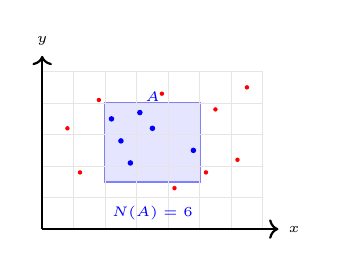
\begin{tikzpicture}[scale=0.4, font=\tiny]

% Define the region A
\filldraw[fill=blue!10, draw=blue!50, thick] (2,1.5) rectangle (5,4);
\node[blue] at (3.5,4.2) {$A$};

% Draw a grid for spatial reference
\draw[gray!20, very thin] (0,0) grid (7,5);

% Axes
\draw[->, thick] (0,0) -- (7.5,0) node[right] {$x$};
\draw[->, thick] (0,0) -- (0,5.5) node[above] {$y$};

% Random points scattered in space
\foreach \x/\y in {1.2/1.8, 2.8/2.1, 3.5/3.2, 1.8/4.1, 4.2/1.3, 
                   3.1/3.7, 2.5/2.8, 4.8/2.5, 5.5/3.8, 6.2/2.2,
                   0.8/3.2, 3.8/4.3, 6.5/4.5, 5.2/1.8, 2.2/3.5} {
    \fill[red] (\x,\y) circle (2pt);
}

% Highlight points inside A
\foreach \x/\y in {2.8/2.1, 3.5/3.2, 3.1/3.7, 2.5/2.8, 2.2/3.5, 4.8/2.5} {
    \fill[blue] (\x,\y) circle (2.5pt);
}

% Count label
\node[blue] at (3.5,0.5) {$N(A) = 6$};

\end{tikzpicture}
};}
\end{tikzpicture}
\end{frame}

\begin{frame}
  \frametitle{History of the Poisson Process}
  1800s:
  \begin{itemize}
  \item Siméon Poisson introduces the Poisson distribution, in 'Research on the probability of judgements in criminal and civil matters'.
    \only<-7>{\item Poisson distribution is a limiting case of the Binomial distribution for rare events.}
  \pause
  \only<-7>{\item Let $X \sim Biniomial(n,p)$ and fix $\lambda=np$,
    \begin{align*}
      \mathbb{P} \{ X=k \}\only<2-5>{&=\textcolor<5>{blue}{\binom{n}{k}} \only<2-3>{\textcolor<3>{blue}{p}^k} \only<4->{\left(\frac{\lambda}{n}\right)^{\textcolor<5>{blue}{k}}} \left(1-\only<2-3>{\textcolor<3>{blue}{p}} \only<4->{\frac{\lambda}{n}}\right)^{n-k} \\}
      \only<5-6>{&= {\left(\frac{n(n-1)...(n-k+1)}{\textcolor<6>{blue}{k!}}\right)}\cdot \left(\frac{\lambda^k}{\textcolor<6>{blue}{n^k}}\right) \cdot \left(1-\frac{\lambda}{n}\right)^{\textcolor<6>{blue}{n-k}} \\}
      \onslide<6-7>{&= \left(\textcolor<7>{blue}{\frac{n(n-1)...(n-k+1)}{n^k}} \cdot \frac{\lambda^k}{k!}\right) \cdot \textcolor<7>{blue}{\left(1-\frac{\lambda}{n}\right)^n} \cdot \textcolor<7>{blue}{\left( 1-\frac{\lambda}{n}\right)^{-k}} \\}
      \onslide<7>{&\to 1 \cdot \frac{\lambda^k}{k!} \cdot e^{-\lambda} \cdot 1}
    \onslide<7>{= \frac{\lambda^k}{k!} \cdot e^{-\lambda} \hspace{1cm} \text{ as } n \to \infty,}
  \end{align*}}
  \only<7>{Hence limit of $X$ as we take $n \to \infty$ is distributed $Poisson(\lambda)$.}
  \pause\pause\pause\pause\pause
    \end{itemize}
  \pause
  1900s:
  \begin{itemize}
    \item Rutherford and others observe properties of radioactive decay and notice:
    \begin{itemize}
    \item Decay events happen at 'random' times.
    \item Waiting time between decay events are distributed exponentially.
    \end{itemize}
  \item Erlang, telecoms engineer known for his contributions to queuing theory, notices:
    \begin{itemize}
    \item Calls arrive at 'random' times.
    \item Length of calls are distributed exponentially.
  \end{itemize}
  \pause
\end{itemize}
  These physicists and engineers were observing the Poisson process.
  1940s:
  \begin{itemize}
    \item Feller gives official definition for the Poisson process. A Poisson process must have the following properties,
    \begin{enumerate}
    \item independent increments,
    \item stationary increments,
    \item probability of multiple events in a small interval is negligable - technicality (automatic if waiting times are distributed exponentially).
    \end{enumerate}
  \end{itemize}
\end{frame}

\begin{frame}
  \frametitle{Poisson Process Definition} 
  \only<1-2>{There are several equivalent definitions of the Poisson process used today one of which is as follows:}

  \begin{itemize}
    \only<1-2>{\item Let $(X_i)_{i\geq0}$ be a sequence of random variables such that waiting times \\$X_i\sim Exponential(\lambda)$ and $\Gamma_n=\sum_{i=0}^n{X_i}$. Then $$N(t):=max\{n:\Gamma_n\leq t\}$$ is a \textit{Poisson process} with rate $\lambda$.}
  \pause
  \item Let $N$ be stochastic process. Then $N$ is a \textit{Poisson process with rate $\lambda$} if
    \begin{enumerate}
    \item $N(0)=0$,
    \item $N$ has independent increments, i.e. for any $0\leq t_0 < ... < t_k$, the random variables, $N(t_1)-N(t_0),...,N(t_n)-N(t_{n-1})$, are independent,   
\item for any $s,t\geq0$, $$N(t+s)-N(s) \sim Poisson(\lambda t),$$
  in particular, $N(t) \sim Poisson(\lambda t).$
  \end{enumerate}
  \end{itemize}

  \pause
\begin{itemize}
\pause
\item We contruct the Poisson process as many Bernoilli arrival 'attempts'. Consider $n$ many intervals of size $h=\frac{t}{n}$, if each interval is distributed approximately Bernoilli: $\mathbb{P} \begin{cases} 1 \text{ arrival } \approx \frac{\lambda t}{n}\\ 0 \text{ arrivals } \approx 1-\frac{\lambda t}{n} \\ > 1 \text{ arrival } \approx 0.\end{cases},$ \\ then the arrivals are distributed approximately $Binomial(n, \frac{\lambda t}{n})$ and $$Binomial \left(n, \frac{\lambda t}{n} \right) \to Poisson(\lambda t).$$

  \end{itemize}
\end{frame}

\begin{frame}
  \frametitle{Generalising the Poisson Process}
  A non-homogeneous Poisson process is a more general form:
  \begin{itemize}
  \item A Poisson process whose rate is not fixed is a non-homogenous Poisson process, its rate is given by the function, $\mu$, the mean measure. Then
    $$N(t) \sim Poisson(\mu (t)).$$
  \end{itemize}

  \pause

  We extend this definition to space:
  \begin{itemize}
    \item Let $\mathcal{E}$ be the class of rectangles in E. Then a point process, $N$ (the function that counts the points in a given set), is a Poisson point process if
    \begin{enumerate} 
      \item for sets $A \in \mathcal{E}$, $$N(A) \sim Poisson(\mu(A)),$$
      \item N is 'completely random', same meaning as independent increments, but for space.
    \end{enumerate}
  \end{itemize}
\end{frame}

\begin{frame}
\frametitle{Order Statistic Property}
A key property of the Poisson process is that given the number of events, $n$, in an interval, the distribution of the time of those events is uniform:
\begin{itemize}
\item If N is a homogeneous Poisson process on $[0,\infty)$ with rate $\lambda$, then 
$$(\Gamma_1,...,\Gamma_n|N(t)=n) \overset{d}{=} (U_{(1)},...,U_{(n)}).$$
\end{itemize}
\pause
This property applies to space:
\begin{itemize}
  \item If mean measure, $\mu$ is a multiple of the Lebesgue measure and given the number of points, $n$, in a set $A$, then the points in that set are distributed Uniformly.
\end{itemize}

\begin{center}
    
\onslide<1->\begin{tikzpicture}[remember picture]
    % Create three separate picture environments for the column    
    \node[anchor=south east] (col2) {

\begin{tikzpicture}[yscale=0.8, xscale=0.9, font=\tiny]

% Main timeline
\draw[<->, thick] (-0.5,0) -- (6.5,0) node[right] {$t$};
\draw[thick] (0,-0.1) -- (0,0.1) node[above] {$0$};
\draw[thick] (6,-0.1) -- (6,0.1) node[above] {$T$};

% Poisson points on timeline
\foreach \x in {0.8, 1.9, 3.2, 4.8, 5.6} {
    \fill[red] (\x,0) circle (3pt);
}

% Label points as order statistics
\node[below] at (0.8,-0.3) {$\Gamma_{1}$};
\node[below] at (1.9,-0.3) {$\Gamma_{2}$};
\node[below] at (3.2,-0.3) {$\Gamma_{3}$};
\node[below] at (4.8,-0.3) {$\Gamma_{4}$};
\node[below] at (5.6,-0.3) {$\Gamma_{5}$};

\node[below] at (0.8,1.2) {$U_{(1)}$};
\node[below] at (1.9,1.2) {$U_{(2)}$};
\node[below] at (3.2,1.2) {$U_{(3)}$};
\node[below] at (4.8,1.2) {$U_{(4)}$};
\node[below] at (5.6,1.2) {$U_{(5)}$};

% Uniform distribution bar above
\draw[thick] (0,1.5) -- (6,1.5);
\draw[thick] (0,1.4) -- (0,1.6) node[left] {$0$};
\draw[thick] (6,1.4) -- (6,1.6) node[right] {$T$};

% Uniform random points
\foreach \x in {0.8, 1.9, 3.2, 4.8, 5.6} {
    \fill[blue] (\x,1.5) circle (2pt);
}

% Sort arrow
\draw[->, thick, gray] (2.7,1) -- node[right] {} (2.7,0.5);

\end{tikzpicture}
};
\onslide<2->\node[anchor=south west] (col5) {
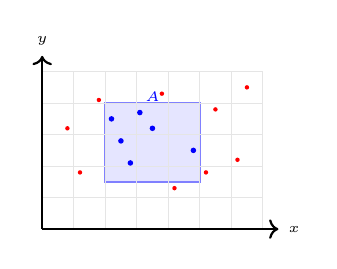
\begin{tikzpicture}[scale=0.4, font=\tiny]

% Define the region A
\filldraw[fill=blue!10, draw=blue!50, thick] (2,1.5) rectangle (5,4);
\node[blue] at (3.5,4.2) {$A$};

% Draw a grid for spatial reference
\draw[gray!20, very thin] (0,0) grid (7,5);

% Axes
\draw[->, thick] (0,0) -- (7.5,0) node[right] {$x$};
\draw[->, thick] (0,0) -- (0,5.5) node[above] {$y$};

% Random points scattered in space
\foreach \x/\y in {1.2/1.8, 2.8/2.1, 3.5/3.2, 1.8/4.1, 4.2/1.3, 
                   3.1/3.7, 2.5/2.8, 4.8/2.5, 5.5/3.8, 6.2/2.2,
                   0.8/3.2, 3.8/4.3, 6.5/4.5, 5.2/1.8, 2.2/3.5} {
    \fill[red] (\x,\y) circle (2pt);
}

% Highlight points inside A
\foreach \x/\y in {2.8/2.1, 3.5/3.2, 3.1/3.7, 2.5/2.8, 2.2/3.5, 4.8/2.5} {
    \fill[blue] (\x,\y) circle (2.5pt);
}

\end{tikzpicture}
};

\end{tikzpicture}

\end{center}

\end{frame}

\begin{frame}
\frametitle{Applying the Poisson Point Process to the Real World}
\begin{itemize}
\item Events that are random and that we can assume are independent can be modelled with Poisson process. Like our example of customers arriving to a cafe.
\item Items that are distributed randomly in space can be modelled with a Poisson point process.
\item We have related this process to the Poisson, Exponential, and Uniform distributions, so we can do lots of calculations about events if we notice they are a Poisson process. 
\item We can calculate the expectations and probabilities of the number of points. We can talk about how they are spread with the order statistic property.
\end{itemize}
\end{frame}
\end{document}
